\chapter{Анализ предметной области} \label{ch1}

\section{White Rabbit} \label{ch1:sec1}

White Rabbit -- система синхронизации часов. Разработана при сотрудничестве множества
институтов и компаний. Изначально проект был начат для улучшения текущей системы синхронизации в Церне (Большой адронный коллайдер).
Предполагалось использование для физических экспериментов, однако в процессе было создано обобщенное решение,
которое нашло своё применение в различных сферах.\\

\noindent Характеристики:

\begin{itemize}
	\item Суб-наносекундная точность
	\item Большое количество синхронизируемых узлов
	\item Расстояния в десятки километров
	\item Канал передачи между двумя узлами –- 1 Gbps
	\item Открытый исходный код\\
\end{itemize}

Достоинствами White Rabbit являются полностью открытый исходный код и аппаратура, а также 
использование существующих стандартов (Ethernet, PTP и т. д.).

\section{Калибровка}

Синхронизация в сети White Rabbit выполняется по протоколу WR PTP (White Rabbit Precison Time Protocol) –- модифицированному протоколу PTP. (IEEE 1588).
Однако для достижения субнаносекундной точности необходима дополнительная калибровка.

Обмен данными между двумя устройствами происходит по одной линии оптоволокна, работающей в полнодуплексном режиме.
Для передачи в одну и другую сторону используется свет с разной длиной волны, поэтому возникает асимметричность в
задержках распространения сигнала. Из-за этого устройство не может само определить задержки, отправив эхо запрос
другому устройству –- время распространения сигнала в одну и другую сторону не равны.

Определение коэффициента асимметричности оптоволокна позволит протоколу White Rabbit PTP обеспечить требуемую точность синхронизации устройств сети.

В [6] описан принцип калибровки и его математическое обоснование.\\

\begin{figure}[ht!] 
	\center
	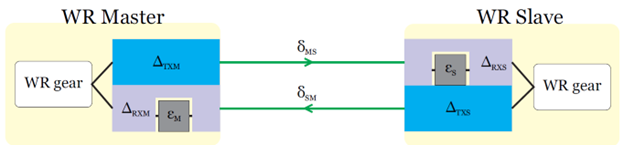
\includegraphics  {my_folder/images//conn_model}
	\caption{Модель соединения между двумя устройствами} 
	\label{fig:conn-model}  
\end{figure}

На \firef{fig:conn-model} изображены возникающие задержки, требующие калибровки. Внутри каждого устройства 
возникают задержки на приёме и отправке ($\Delta_{TXM},\Delta_{RXM},\Delta_{TXS},\Delta_{RXS}, \varepsilon_{M},\varepsilon_{S}$),
которые являются результатом задержек в SFP (Small Form-factor Pluggable) 
модуле, в электрических цепях и электронных компонентах. Эти задержки калибруются отдельно на каждом устройстве при помощи loopback петли и не являются
предметом рассмотрения в данной работе.

Суммарная задержка распространения сигнала от ведущего устройства к ведомому устройству и обратно считается по формуле:

\begin{equation}
delay_{MM} = \Delta_{TXM} + \Delta_{RXS} + \varepsilon_{S} + \Delta_{TXS} + \Delta_{RXM} + \varepsilon_{M} + \delta_{MS} + \delta_{SM}
\end{equation}

В ходе данной работы разрабатывается устройство для калибровки коэффициента асимметричности.

Коэффициент асимметричности определяется, как:

\begin{equation}
	\alpha = \frac{\delta_{MS} - \delta_{SM}}{\delta_{SM}}
\end{equation}

Измеряется коэффициент при помощи дополнительного короткого оптоволокна, с известной задержкой (\firef{fig:meas-scheme-1}).

\begin{figure}[ht!] 
	\center
	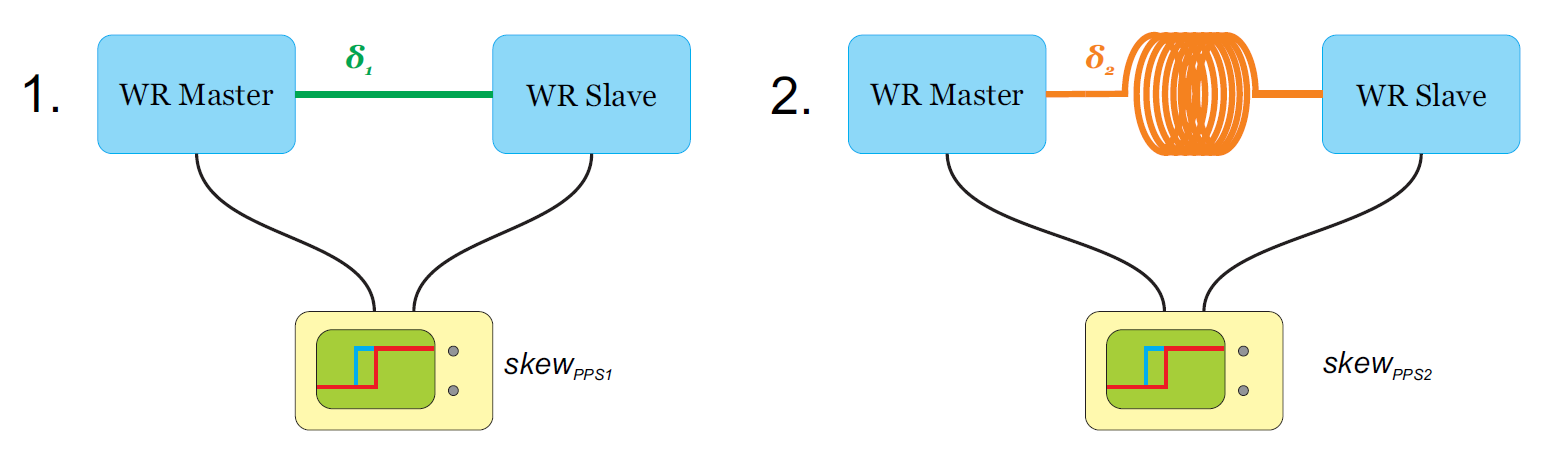
\includegraphics [scale=0.4] {my_folder/images//meas_scheme_1}
	\caption{Измерение асимметричности про помощи дополнительного оптоволокна} 
	\label{fig:meas-scheme-1}  
\end{figure}

Два устройства подключаются калибруемым оптоволокном ($\delta_{2}$) и дополнительным ($\delta_{1}$) отдельно, 
далее два устройства синхронизируются. После этого измеряется разность фаз синхросигналов 1-PPS
(Pulse Per Second)($ skew_{PPS} $), генерируемых ведущим и ведомым устройством. 

\begin{equation}
	skew_{PPS} = t_{PPS_S} - t_{PPS_M}\\
\end{equation}

Подставив измеренные значения в формулу \labelcref{eq:alpha} можно вычислить искомый коэффициент асимметричности.\\

\begin{equation}
	\label{eq:alpha}
	\alpha = \frac{2 \left( skew_{PPS2} - skew_{PPS1} \right) }{\frac{1}{2} \delta_2 - \left( skew_{PPS2} - skew_{PPS1} \right)}\\
\end{equation}

\bigbreak

Вышеописанный метод подходит для случаев, когда линия оптоволокна ещё не установлена.
В иных случаях применяется немного изменённый метод с подключением петли от выхода 1-PPS одного устройства к другому (\firef{fig:meas-scheme-2}). 
Измеряется расхождение фаз при передачи сигнала PPS от одного устройства и от другого. Полученные значения усредняются (\labelcref{eq:skew_mean}).

\begin{figure}[ht!] 
	\center
	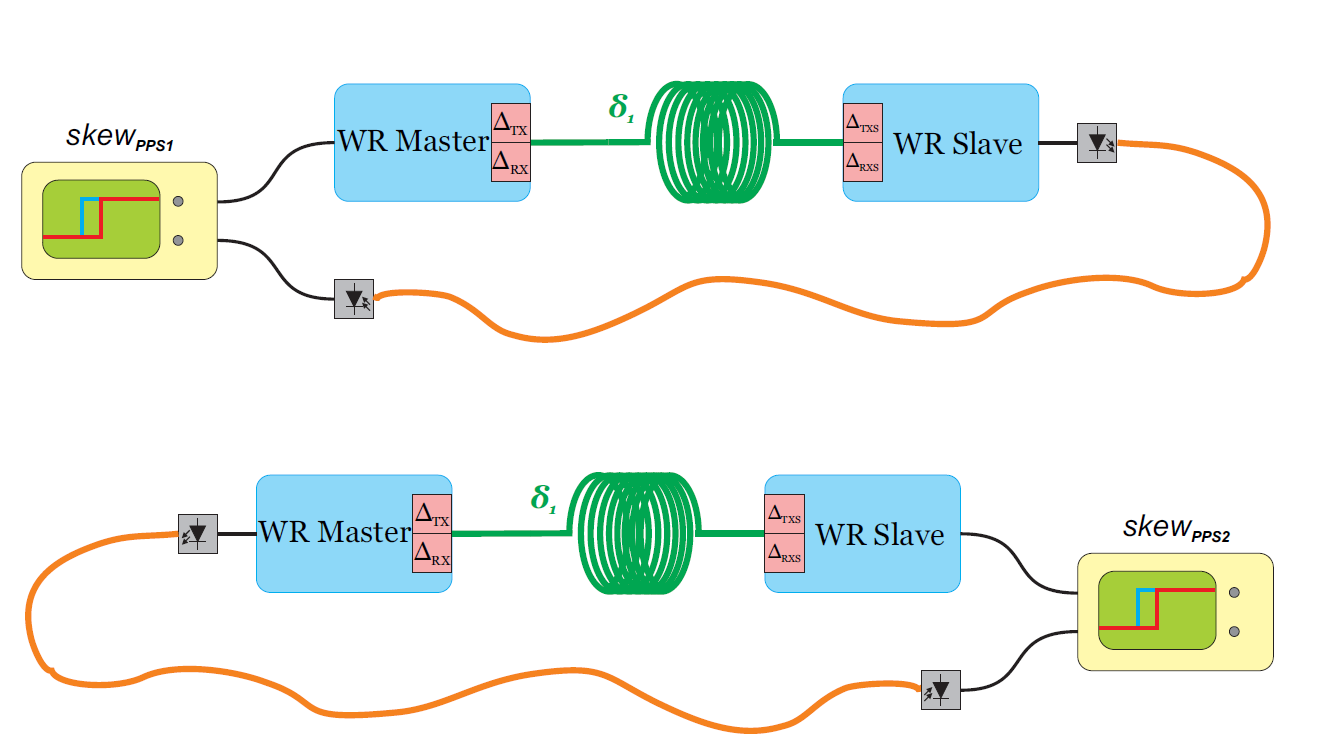
\includegraphics [scale=0.4] {my_folder/images//meas_scheme_2}
	\caption{Измерение асимметричности установленной линии} 
	\label{fig:meas-scheme-2}  
\end{figure}

\begin{equation}
	\label{eq:skew_mean}
	skew_{PPS} = \frac{1}{2} \left(skew_{PPS1} + skew_{PPS2} \right)
\end{equation}

Далее это значение может быть использовано для вычисления коэффициента по формуле \labelcref{eq:alpha}. Однако для данного метода так же требуется
короткое оптоволокно с известной задержкой.

\section{Актуальность}

Для процесса калибровки предполагается использовать устройство, способное измерять отрезки времени меньше, чем 1 нс, чтобы обеспечить
субнаносекундную точность, т.е. иметь частоту дискретизации 1 GSa. Если применить правило <<пятикратного превышения частоты дискретизации>>, то
используемый осциллограф должен иметь частоту дискретизации выше 5 GSa. 

Цена осциллографов с такими характеристиками крайне высока. Актуальность данной работы заключается в том, что предлагается разработать
относительно бюджетное устройство, работающее по принципу стробоскопического осциллографа.
 
Сигналы PPS от калибруемых устройств являются периодическими. Это позволяет применить для их обнаружения, захвата и анализа устройство,
работающее по принципу стробоскопического осциллографа.

\section{Стробоскопический осциллограф}

Стробоскопические осциллографы предназначены для обнаружения, захвата и анализа периодических сигналов.
Принцип работы стробоскопического осциллографа проиллюстрирован на \firef{fig:stb-osc}.

\begin{figure}[ht!] 
	\center
	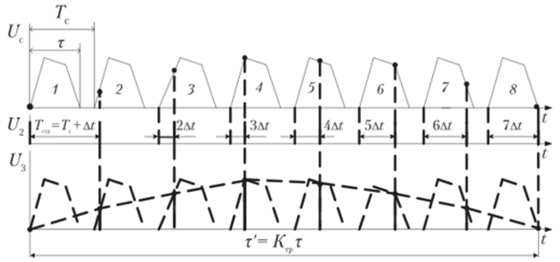
\includegraphics {my_folder/images//stb_osc}
	\caption{Принцип работы стробоскопического осциллографа} 
	\label{fig:stb-osc}  
\end{figure}
\newpage

\noindent Условные обозначения:

\begin{itemize}[label={}]
	\item $ U_{c} $ -- исследуемый периодический сигнал
	\item $ T_{c} $ -- период исследуемого сигнала
	\item $ \tau $ -- длительность исмпульса исследуемого сигнала
	\item $ \Delta t $ -- шаг считывания исследуемого сигнала
	\item $ U_{2} $ -- стробы осциллографа
	\item $ U_{3} $ -- снятая осциллограмма сигнала\\
\end{itemize}

Таким образом, для снятия очередной точки изменяется смещение $ \Delta t $.
Частота дискретизации определяется минимальным смещением, которое может задать осциллограф.\\

\noindent Осциллограмма исследуемого сигнала снимается следующим образом:

\begin{itemize}
    \item[1.] Осциллограф захватывает группу выборок измеряемого сигнала $ U_{c} $ с периодом $ T $
    \item[2.] Осциллограф смещает точку запуска на величину $ \Delta t $ и захватывает следующий набор выборок
    \item[3.] Процесс повторяется, в результате чего строится осциллограмма сигнала\\
\end{itemize}
	
Описанный принцип действия стробоскопических осциллографов обеспечивает высокую чувствительность и широкую полосу пропускания этих приборов.
Ключевое значение для работы стробоскопического осциллографа имеет шаг сдвига точки захвата сигнала.
Частота дискретизации при этом становится не столь несущественна. Большой объём памяти также не требуется,
так требуется захватывать и обрабатывать малое число выборок.


\FloatBarrier
\newpage